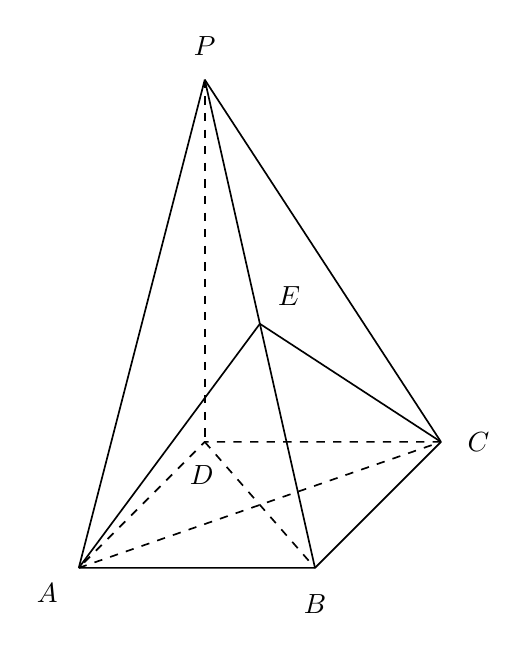
\begin{tikzpicture}[x=1cm,y=1cm,line width=.6pt,font=\normalsize]
% Schematic pyramid; base square oblique, apex above D side
\coordinate (A) at (0,0);
\coordinate (B) at (3,0);
\coordinate (C) at (4.6,1.6);
\coordinate (D) at (1.6000000000,1.6000000000);
\coordinate (P) at (1.6000000000,6.2000000000);
\coordinate (E) at (2.3000000000,3.1000000000);
% base
\draw (A)--(B)--(C);
\draw[dashed] (C)--(D)--(A);
\draw[dashed] (A)--(C);
\draw[dashed] (D)--(B);
% lateral edges
\draw (P)--(A);
\draw (P)--(E)--(B);
\draw (P)--(C);
\draw[dashed] (P)--(D);
% section AEC
\draw (A)--(E);
\draw (E)--(C);
% labels with clearance
\node[anchor=north east,xshift=-4pt,yshift=-2pt] at (A) {$A$};
\node[anchor=north,yshift=-6pt] at (B) {$B$};
\node[anchor=west,xshift=6pt] at (C) {$C$};
\node[anchor=north west,xshift=-9pt,yshift=-5pt] at (D) {$D$};
\node[anchor=south,yshift=5pt] at (P) {$P$};
\node[anchor=south west,xshift=3pt,yshift=3pt] at (E) {$E$};
\end{tikzpicture}
